%  article.tex (Version 3.3, released 19 January 2008)
%  Article to demonstrate format for SPIE Proceedings
%  Special instructions are included in this file after the
%  symbol %>>>>
%  Numerous commands are commented out, but included to show how
%  to effect various options, e.g., to print page numbers, etc.
%  This LaTeX source file is composed for LaTeX2e.

%  The following commands have been added in the SPIE class 
%  file (spie.cls) and will not be understood in other classes:
%  \supit{}, \authorinfo{}, \skiplinehalf, \keywords{}
%  The bibliography style file is called spiebib.bst, 
%  which replaces the standard style unstr.bst.  

\documentclass[a4paper]{spie}  %>>> use for US letter paper
%%\documentclass[a4paper]{spie}  %>>> use this instead for A4 paper
%%\documentclass[nocompress]{spie}  %>>> to avoid compression of citations
%% \addtolength{\voffset}{9mm}   %>>> moves text field down
%% \renewcommand{\baselinestretch}{1.65}   %>>> 1.65 for double spacing, 1.25 for 1.5 spacing 
%  The following command loads a graphics package to include images 
%  in the document. It may be necessary to specify a DVI driver option,
%  e.g., [dvips], but that may be inappropriate for some LaTeX 
%  installations. 
\usepackage{wrapfig}
\usepackage{ragged2e}
\usepackage{graphicx}
\usepackage{color}   %May be necessary if you want to color links
\usepackage{hyperref}
\hypersetup{
    colorlinks=true, %set true if you want colored links
    linktoc=all,     %set to all if you want both sections and subsections linked
    linkcolor=blue,  %choose some color if you want links to stand out
}

\title{\uppercase{ {\fontsize{120}{120}\selectfont La vie est dr\"{o}le}} \\ 
\bigskip \bigskip \bigskip \bigskip
{\fontsize{40}{40}\selectfont Fichero Recetario}}


%>>>> The author is responsible for formatting the 
%  author list and their institutions.  Use  \skiplinehalf 
%  to separate author list from addresses and between each address.
%  The correspondence between each author and his/her address
%  can be indicated with a superscript in italics, 
%  which is easily obtained with \supit{}.

\author{Mart\'in Aversa \\
Sebasti\'an Aversa \\
Eli C\'espedes \\
Iv\'an Garcia \\
Nicol\'as Gonzalez \\
Alejandro Montes de Oca \\
Lucas V\'elez
\skiplinehalf}

%>>>> Further information about the authors, other than their 
%  institution and addresses, should be included as a footnote, 
%  which is facilitated by the \authorinfo{} command.

\authorinfo{Autores: \\ Mart\'in Aversa \\
Sebasti\'an Aversa \\
Eli C\'espedes \\
Iv\'an Garcia \\
Nicol\'as Gonzalez \\
Alejandro Montes de Oca \\
Lucas V\'elez}
%%>>>> when using amstex, you need to use @@ instead of @
 
%%%%%%%%%%%%%%%%%%%%%%%%%%%%%%%%%%%%%%%%%%%%%%%%%%%%%%%%%%%%% 
%>>>> uncomment following for page numbers
\pagestyle{plain}    
%>>>> uncomment following to start page numbering at 301 
\setcounter{page}{2} 
 
\begin{document} 
  \maketitle 

%%%%%%%%%%%%%%%%%%%%%%%%%%%%%%%%%%%%%%%%%%%%%%%%%%%%%%%%%%%%%
\section{INTRODUCCI\'ON}
\label{sec:intro}  % \label{} allows reference to this section

Este documento describe los ingredientes, proporciones y m\'etodos para realizar distintos cocteles.
\bigskip
\bigskip
%%%%%%%%%%%%%%%%%%%%%%%%%%%%%%%%%%%%%%%%%%%%%%%%%%%%%%%%%%%%%
\tableofcontents

\newpage
\section{Cocteles ingleses}
\bigskip \bigskip \bigskip
\subsection{Born to be British}
\bigskip 
\bigskip 
\subsubsection{Contenido}
\bigskip 
%\begin{wrapfigure}{r}{0.5\textwidth}
%  \begin{center}
%    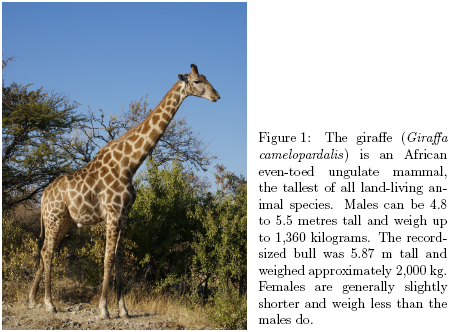
\includegraphics[width=0.48\textwidth]{./ingles/Latex_example_sidecap.jpg}
%  \end{center}
%\end{wrapfigure}

\begin{description}
\item[Nombre:] Born to be British
\item[Cristaleria:] Rock glass (6oz / 180cc)
\item[M\'etodo de elaboraci\'on:] Batido
\item[Decoraci\'on:] Rodajas de manzana
\end{description}

\begin{table}[h]
\caption{Ingredientes y proporciones} 
\label{tab:fonts}
\begin{center}       
\begin{tabular}{|l|l|l|c|l|} %% this creates two columns
%% |l|l| to left justify each column entry
%% |c|c| to center each column entry
%% use of \rule[]{}{} below opens up each row
\hline
\rule[-1ex]{0pt}{3.5ex}  \textbf{Producto} & \textbf{Bebida} & \textbf{Marca} & \textbf{Volumen} & \textbf{Fraccion}  \\
\hline
\rule[-1ex]{0pt}{3.5ex}  Aguardiente & Gin 			& Boodles British 		& 1  $\frac{1}{2}$ oz / 45 cc 	&  	\\
\hline
\rule[-1ex]{0pt}{3.5ex}  Licor 		& Triple Sec 	& Cointreau 				& $\frac{1}{4}$ oz / 7,5 cc 		&  	\\
\hline
\rule[-1ex]{0pt}{3.5ex}  Fruta 		& Manzana roja 	& Jugo	 				& 2 oz / 60 cc					& 	\\
\hline
\rule[-1ex]{0pt}{3.5ex}  Fruta 		& Manzana roja 	& Gajos (s/ c\'ascara)	& 4								& 	\\
\hline
\rule[-1ex]{0pt}{3.5ex}  Fruta 		& Manzana roja 	& Gajos chicos (s/ c\'ascara)	& 3								& 	\\
\hline
\rule[-1ex]{0pt}{3.5ex}  Fruta 		& lim\'on	 	& Gajos (s/ c\'ascara ni piel)	& 2								& 	\\
\hline
\rule[-1ex]{0pt}{3.5ex}  Jarabe		& Simple Syrup 	& 						& $\frac{3}{4}$ oz / 22,5 cc 		&  	\\
\hline
\end{tabular}
\end{center}
\end{table} 
Simple Syrup: 1 parte de agua y 1 parte de az\'ucar.
\bigskip 

%%-----------------------------------------------------------
\subsubsection{Formato de elaboraci\'on} 
\label{sec:title}
\bigskip 
\begin{center}
\begin{enumerate}
\item Colocar los gajos grandes de manzana y los de lim\'on en la coctelera.
\item Colocar el triple sec y el alm\'ibar en la coctelera.
\item Revolver estos ingredientes.
\item Agregar hielo en la coctelera.
\item Agregar el jugo de manzana y el gin.
\item Tapar la coctelera y batir.
\item Servir en vaso Rock Glass.
\item Decorar con los 3 gajos chicos de manzana. Dos pueden ir dentro del trago y el otro en el borde del vaso.
\end{enumerate}
\end{center}
\bigskip 
\bigskip 
%%%%%%%%%%%%%%%%%%%%%%%%%%%%%%%%%%%%%%%%%%%%%%%%%%%%%%%%%%%%%

\subsubsection{Notas}
\bigskip 
\begin{center}
\raggedright{}Servir sin sorbete.
\end{center} 

%\subsubsection{Informaci\'on extra}
\bigskip
%\begin{center}
\medskip 
%\raggedright{ \textbf{Or\'igenes de este trago}} \\ 
\medskip


%\end{center}
\newpage

\newpage
\bigskip \bigskip \bigskip
\subsection{Gin \& Tonic}
\bigskip 
\bigskip 
 
\subsubsection{Contenido}
\bigskip 
\begin{description}
\item[Nombre:] Gin \& Tonic
\item[Cristaleria:] Rock glass (6oz / 180cc)
\item[M\'etodo de elaboraci\'on:] Directo
\item[Decoraci\'on:] Rodajas de lima
\end{description}

\begin{table}[h]
\caption{Ingredientes y proporciones} 
\label{tab:fonts}
\begin{center}       
\begin{tabular}{|l|l|l|c|l|} %% this creates two columns
%% |l|l| to left justify each column entry
%% |c|c| to center each column entry
%% use of \rule[]{}{} below opens up each row
\hline
\rule[-1ex]{0pt}{3.5ex}  \textbf{Producto} & \textbf{Bebida} & \textbf{Marca} & \textbf{Volumen} & \textbf{Fraccion}  \\
\hline
\rule[-1ex]{0pt}{3.5ex}  Aguardiente & Gin 			& Boodles British 		& 2 oz / 60 cc 	&  	\\
\hline
\rule[-1ex]{0pt}{3.5ex}  Gaseosa		& Agua t\'onica 	& Schweppes 				& 4 oz / 120 cc 		&  	\\
\hline
\rule[-1ex]{0pt}{3.5ex}  Fruta 		& Lim\'on	 	& Exprimido				& $\frac{1}{2}$	lim\'on		& 	\\
\hline
\rule[-1ex]{0pt}{3.5ex}  Fruta 		& Lima		 	& 						& 1 rodaja		& 	\\
\hline
\end{tabular}
\end{center}
\end{table} 
\bigskip 

%%-----------------------------------------------------------
\subsubsection{Formato de elaboraci\'on} 
\label{sec:title}
\bigskip 
\begin{center}
\begin{enumerate}
\item Llenar un vaso Rock Glass con hielo.
\item Exprimir medio lim\'on en el vaso.
\item A\~nadir el gin y completar con el agua t\'onica.
\item Decorar con la rodaja de lima.
\end{enumerate}
\end{center}
\bigskip \bigskip 
\bigskip 
%%%%%%%%%%%%%%%%%%%%%%%%%%%%%%%%%%%%%%%%%%%%%%%%%%%%%%%%%%%%%

\subsubsection{Notas}
\bigskip 
\begin{center}
\raggedright{}Servir con sorbete.
\end{center} 
\bigskip \bigskip \bigskip 
\subsubsection{Informaci\'on extra}
\bigskip
\begin{center}

\medskip 
\raggedright{ \textbf{Or\'igenes de este trago}} \\ 
\medskip

{\justifying{
El origen del gin-tonic se sit\'ua en India, en el siglo XIX. Fue en la \'epoca, de expansi\'on territorial de Inglaterra. Durante su paso por India, donde predominaba la malaria, los colonos brit\'anicos tomaban quinina para evitar contagiarse. Preparaban una mezcla con quinina, agua y aromatizantes. M\'as tarde, Cadbury Schweppes (conocida hoy en d\'ia por sus bebidas gasificadas) sustituy\'o el agua por soda, para hacerla m\'as digerible, y crearon as\'i la ''Indian Water Tonic''. \\
\indent Para hacer la bebida m\'as rica, los soldados brit\'anicos, le a\~{n}adieron alcohol: la ginebra Bombay destilada en la ciudad del mismo nombre. As\'i nace el gin-tonic. En poco tiempo la mezcla pas\'o de ser una medicina preventiva a una bebida refrescante y social hasta el punto que en el a\~no 1870 la mezcla de Indian Water Tonic con ginebra era m\'as que conocida.\\ 
\indent Actualmente es una de las bebidas m\'as conocidas y consumidas del mundo y la podemos encontrar en cualquier bar al que vayamos.

La quinina es un alcaloide extra\'ido de la corteza del Quino. Es de sabor muy amargo con propiedades curativas. Anti\"{u}amente era utilizado para tratar la malaria, hasta que fue reemplazado por medicamentos sint\'eticos m\'as eficaces.
}\par}
\end{center}
\newpage

\newpage
\section{Cocteles franceses}
\bigskip \bigskip \bigskip
\subsection{French 75}
\bigskip 
\bigskip 
 
\subsubsection{Contenido}
\bigskip 
\begin{description}
\item[Nombre:] French 75
\item[Cristaleria:] Vaso de champagne (5oz / 150cc)
\item[M\'etodo de elaboraci\'on:] Batido
\item[Decoraci\'on:] C\'ascara de lim\'on cortada en espiral
\end{description}

\begin{table}[h]
\caption{Ingredientes y proporciones} 
\label{tab:fonts}
\begin{center}       
\begin{tabular}{|l|l|l|c|l|} %% this creates two columns
%% |l|l| to left justify each column entry
%% |c|c| to center each column entry
%% use of \rule[]{}{} below opens up each row
\hline
\rule[-1ex]{0pt}{3.5ex}  \textbf{Producto} & \textbf{Bebida} & \textbf{Marca} & \textbf{Volumen} & \textbf{Fracci\'on}  \\
\hline
\rule[-1ex]{0pt}{3.5ex}  Aguardiente & Gin 			& Boodles British 		& 1 $\frac{1}{2}$ oz / 45 cc 	&  	\\
\hline
\rule[-1ex]{0pt}{3.5ex}  Espumante	& Champage Brut 	& Cristal 				& 3 oz / 80 cc 		&  	\\
\hline
\rule[-1ex]{0pt}{3.5ex}  Fruta 		& Lim\'on	 	& Exprimido				& $\frac{1}{2}$	oz		& 	\\
\hline
\rule[-1ex]{0pt}{3.5ex}  Fruta 		& Lim\'on	 	& C\'ascara				& ANP			& 	\\
\hline
\rule[-1ex]{0pt}{3.5ex}  Az\'ucar 		& 			 	& 					& 1 cdita		& 	\\
\hline
\end{tabular}
\end{center}
\end{table} 
1 cdita de az\'ucar = $\frac{1}{2}$ oz = 5gr.
\bigskip 

%%-----------------------------------------------------------
\subsubsection{Formato de elaboraci\'on} 
\label{sec:title}
\bigskip 
\begin{center}
\begin{enumerate}
\item Llenar un vaso de champagne con hielo.
\item Colocar hielo picado en una coctelera.
\item Colocar el gin, el lim\'on y el champagne en la coctelera.
\item Tapar la coctelera y batir.
\item Colar y servir en el vaso del paso 1.
\item Decorar el vaso con la c\'ascara de lim\'on cortada en espiral.
\end{enumerate}
\end{center}
\bigskip \bigskip 
\bigskip 
%%%%%%%%%%%%%%%%%%%%%%%%%%%%%%%%%%%%%%%%%%%%%%%%%%%%%%%%%%%%%

\subsubsection{Notas}
\bigskip 
\begin{center}
\raggedright{}Servir sin sorbete.
\end{center} 
\bigskip \bigskip \bigskip 
\subsubsection{Informaci\'on extra}
\bigskip
\begin{center}

\medskip 
\raggedright{ \textbf{Or\'igenes de este trago}} \\ 
\medskip

{\justifying{
Este trago cuenta con diversas versiones de su origen. Entre ellas: \\

\medskip

\textbf{Primera historia} \\

La bebida fue creada en 1915 en el Harry’s New York Bar de Par\'is, por el barman mundialmente conocido, Harry MacElhone, es muy probable que en el Harry’s New York Bar, fuera donde el coñac se reemplazara por la ginebra, debido a que el bar, el m\'as emblem\'atico del Par\'is de principios del siglo pasado, era el lugar preferido de la American Field Ambulance Service Corps, y de otros muchos estadounidenses que por este tiempo viv\'ian en Par\'is, entre los que cabe destacar a los escritores Francis Scott Fitzgerald y Ernest Hemingway, ambos reconocidos aficionados de la cocteler\'ia. M\'as tarde el c\'octel French 75 llegar\'ia a los Estados Unidos y fue popularizado en el Stork Club de Nueva York.

\bigskip

\textbf{Segunda historia} \\

\indent La bebida fue creada durante la Primera Guerra Mundial originalmente por Raoul Lufbery, un famoso piloto franco-estadounidense. Lufbery pertenec\'ia a la Escadrille Am\'ericaine, tambi\'en conocida como la Escuadrilla Lafayette. Cuenta la leyenda que a Raoul Lufbery le gustaba el champagne pero despu\'es de las misiones de combate necesitaba algo m\'as potente, por lo que decidi\'o añadirle co\~nac, ya que este ingrediente en Francia era f\'acil de conseguir. \\
\indent El c\'octel era tan fuerte que supuestamente ten\'ia tanta potencia como los proyectiles que lanzaba el famoso ca\~n\'on de campa\~na M1897 de 75 mm, orgullo de la artiller\'ia de campa\~na francesa durante la Primera Guerra Mundial. El ca\~n\'on de tiro r\'apido y con un mecanismo de retroceso hidroneum\'atico, en su tiempo la pieza m\'as moderna de la artillería francesa, tambi\'en era conocido como “Franc\'es 75” o “Soixante Quinze” en franc\'es, de ah\'i que Raoul Lufbery decidiera bautizar al c\'octel en cuesti\'o como Franc\'es 75, en honor a la sofisticada pieza de artiller\'ia del ejercito franc\'es.

}\par}
\end{center}
\newpage

\newpage
\bigskip \bigskip \bigskip
\subsection{Sidecar}
\bigskip 
\bigskip 
\subsubsection{Contenido}
\bigskip 
%\begin{wrapfigure}{r}{0.5\textwidth}
%  \begin{center}
%    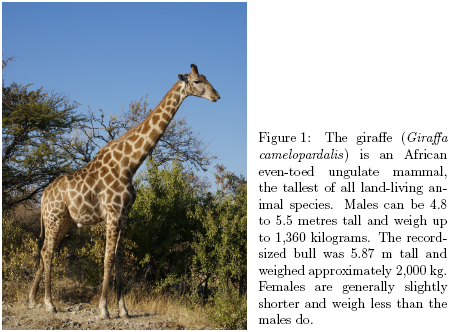
\includegraphics[width=0.48\textwidth]{./ingles/Latex_example_sidecap.jpg}
%  \end{center}
%\end{wrapfigure}

\begin{description}
\item[Nombre:] Sidecar
\item[Cristaleria:] Copa de cognac (5oz / 150cc)
\item[M\'etodo de elaboraci\'on:] Batido
\item[Decoraci\'on:] c\'ascara de lim\'on espiralada
\end{description}

\begin{table}[h]
\caption{Ingredientes y proporciones} 
\label{tab:fonts}
\begin{center}       
\begin{tabular}{|l|l|l|c|l|} %% this creates two columns
%% |l|l| to left justify each column entry
%% |c|c| to center each column entry
%% use of \rule[]{}{} below opens up each row
\hline
\rule[-1ex]{0pt}{3.5ex}  \textbf{Producto} & \textbf{Bebida} & \textbf{Marca} & \textbf{Volumen} & \textbf{Fracci\'on}  \\
\hline
\rule[-1ex]{0pt}{3.5ex}  Brandy		& Cognac			& Hennessy		 		& 1  $\frac{1}{2}$ oz / 45 cc 	&  	\\
\hline
\rule[-1ex]{0pt}{3.5ex}  Licor 		& Triple Sec 	& Cointreau 				& $\frac{3}{4}$ oz / 37,5 cc 		&  	\\
\hline
\rule[-1ex]{0pt}{3.5ex}  Fruta 		& Lim\'on	 	& Jugo	 				& 3 oz / 60 cc					& 	\\
\hline
\end{tabular}
\end{center}
\end{table} 
\bigskip 

%%-----------------------------------------------------------
\subsubsection{Formato de elaboraci\'on} 
\label{sec:title}
\bigskip 
\begin{center}
\begin{enumerate}
\item Impregnar el borde del vaso de cognac en az\'ucar.
\item Colocar hielo en una coctelera.
\item Colocar el triple sec, el cognac y el jugo de lim\'on en la coctelera.
\item Tapar la coctelera y batir.
\item Servir en el vaso de cognac.
\item Decorar con la tira de c\'ascara de lim\'on.
\end{enumerate}
\end{center}
\bigskip 
\bigskip 
%%%%%%%%%%%%%%%%%%%%%%%%%%%%%%%%%%%%%%%%%%%%%%%%%%%%%%%%%%%%%

\subsubsection{Notas}
\bigskip 
\begin{center}
\raggedright{}Servir sin sorbete.
\end{center} 

\subsubsection{Informaci\'on extra}
\bigskip
\begin{center}
\medskip 
\raggedright{ \textbf{Or\'igenes de este trago}} \\ 
\medskip

{\justifying{
\indent La creaci\'on del cocktail se le atribuye a Harry MacElhone (tambi\'en creador del Brandy Alexander o el White Lady) a finales de la primera Guerra Mundial.
Se comenta que el nombre del cocktail surge por un capit\'an del ej\'ercito que todas las noches ped\'ia esta bebida para combatir el resfriado y el fr\'io, sus efectos eran tan fuertes que ten\'ian que llevarlo a su casa en Sidecar. \\

\indent Son varios los que se atribuyen la creaci\'on de este cocktail, el propio MacElhone en su libro Harry’s ABC of Mixing Cocktails le atribuy\'o el m\'erito a Pat MacGarry, un barman londinense. Tambi\'en el Hotel Ritz reclama la creaci\'on del Sidecar.
}\par}
\end{center}
\newpage

\newpage
\section{Cocteles italianos}
\bigskip \bigskip \bigskip
\subsection{Negroni}
\bigskip 
\bigskip 
\subsubsection{Contenido}
\bigskip 
%\begin{wrapfigure}{r}{0.5\textwidth}
%  \begin{center}
%    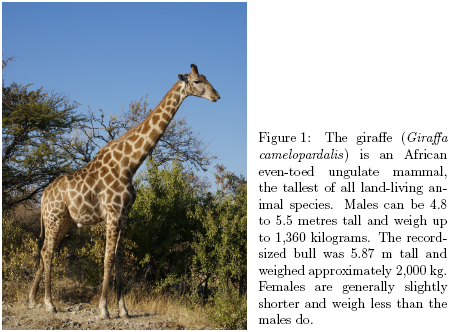
\includegraphics[width=0.48\textwidth]{./ingles/Latex_example_sidecap.jpg}
%  \end{center}
%\end{wrapfigure}

\begin{description}
\item[Nombre:] Negroni
\item[Cristaleria:] Rock glass (6oz / 180cc)
\item[M\'etodo de elaboraci\'on:] Batido
\item[Decoraci\'on:] C\'ascara de naranja
\end{description}

\begin{table}[h]
\caption{Ingredientes y proporciones} 
\label{tab:fonts}
\begin{center}       
\begin{tabular}{|l|l|l|c|l|} %% this creates two columns
%% |l|l| to left justify each column entry
%% |c|c| to center each column entry
%% use of \rule[]{}{} below opens up each row
\hline
\rule[-1ex]{0pt}{3.5ex}  \textbf{Producto} & \textbf{Bebida} & \textbf{Marca} & \textbf{Volumen} & \textbf{Fraccion}  \\
\hline
\rule[-1ex]{0pt}{3.5ex}  Aguardiente & Gin 			& Boodles British 		& 1 oz / 30 cc 	&  	\\
\hline
\rule[-1ex]{0pt}{3.5ex}  Licor 		& Campari	 	& 				& 1 oz / 30 cc 		&  	\\
\hline
\rule[-1ex]{0pt}{3.5ex}  Vermouth	& Cinzano Rosso 	& Cinzano 				& 1 oz / 30 cc					& 	\\
\hline
\rule[-1ex]{0pt}{3.5ex}  Fruta 		& Naranja		& C\'ascara		& 								& 	\\
\hline
\end{tabular}
\end{center}
\end{table} 
\bigskip 

%%-----------------------------------------------------------
\subsubsection{Formato de elaboraci\'on} 
\label{sec:title}
\bigskip 
\begin{center}
\begin{enumerate}
\item Colocar hielo en una coctelera.
\item Colocar el gin, campari y cinzano en la coctelera.
\item Tapar la coctelera y batir.
\item Servir en vaso Rock Glass.
\item Aromatizar y decorar con la c\'ascara de naranja.
\end{enumerate}
\end{center}
\bigskip 
\bigskip 
%%%%%%%%%%%%%%%%%%%%%%%%%%%%%%%%%%%%%%%%%%%%%%%%%%%%%%%%%%%%%

\subsubsection{Notas}
\bigskip 
\begin{center}
\raggedright{}Servir con sorbete.
\end{center} 

\subsubsection{Informaci\'on extra}
\bigskip
\begin{center}
\medskip 
\raggedright{ \textbf{Or\'igenes de este trago}} \\ 
\medskip

{\justifying{
\indent El Negroni, cuyo nombre refiere al apellido de su creador el Conde Camilo Negroni, se invent\'o aproximadamente en el a\~no 1920, en Florencia. El c\'octel preferido del se\~nor Negroni era el Americano, pero el cre\'ia que a\'un pod\'ia ser mejor y m\'as fuerte, por eso le pidi\'o a su cantinero que sustituyese la soda por gin, y as\'i naci\'o el Negroni, un trago espectacular. Este trago se considera como un excelente aperitivo y uno de los tragos m\'as importantes de Italia.
}\par}
\end{center}
\newpage

\newpage
\bigskip \bigskip \bigskip
\subsection{Martini}
\bigskip 
\bigskip 
\subsubsection{Contenido}
\bigskip 
%\begin{wrapfigure}{r}{0.5\textwidth}
%  \begin{center}
%    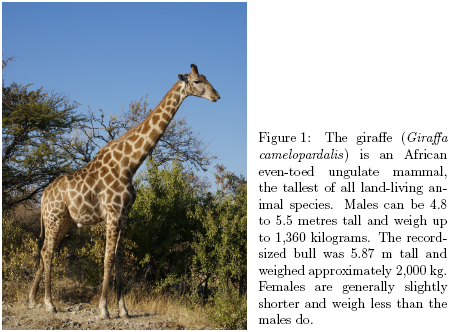
\includegraphics[width=0.48\textwidth]{./ingles/Latex_example_sidecap.jpg}
%  \end{center}
%\end{wrapfigure}

\begin{description}
\item[Nombre:] Martini Seco
\item[Cristaleria:] Copa Cóctel (4oz / 120cc)
\item[M\'etodo de elaboraci\'on:] Revuelto
\item[Decoraci\'on:] Aceituna
\end{description}

\begin{table}[h]
\caption{Ingredientes y proporciones} 
\label{tab:fonts}
\begin{center}       
\begin{tabular}{|l|l|l|c|l|} %% this creates two columns
%% |l|l| to left justify each column entry
%% |c|c| to center each column entry
%% use of \rule[]{}{} below opens up each row
\hline
\rule[-1ex]{0pt}{3.5ex}  \textbf{Producto} & \textbf{Bebida} & \textbf{Marca} & \textbf{Volumen} & \textbf{Fraccion}  \\
\hline
\rule[-1ex]{0pt}{3.5ex}  Aguardiente & Ginebra seca 			& Schlichte 		& 3 oz / 90 cc 	&  	\\
\hline
\rule[-1ex]{0pt}{3.5ex}  Vermouth 		& Cinzano Rosso 	& Cinzano 				& 1 oz / 30 cc 		&  	\\
\hline
\rule[-1ex]{0pt}{3.5ex}  Fruta 		& Limon & Gajo (s/ c\'ascara)	& 1		& 	\\
\hline
\rule[-1ex]{0pt}{3.5ex}  Fruta 		& Aceituna & Finca Cave Canem (s/ c\'ascara)	& 1		& 	\\
\hline
\end{tabular}
\end{center}
\end{table} 
\bigskip 

%%-----------------------------------------------------------
\subsubsection{Formato de elaboraci\'on} 
\label{sec:title}
\bigskip 
\begin{center}
\begin{enumerate}
\item Colocar en un vaso de composición 5 hielos, el vermouth, la ginebra y 10 gotas de lim\'on.
\item Revolver con la cucharilla mezcladora logrando que el l\'iquido se enfr\'ie.
\item Con un colador servir en la copa coctail, evitando servir el hielo.
\item Agregar una aceituna a la copa.

\end{enumerate}
\end{center}
\bigskip 
\bigskip 
%%%%%%%%%%%%%%%%%%%%%%%%%%%%%%%%%%%%%%%%%%%%%%%%%%%%%%%%%%%%%

\subsubsection{Notas}
\bigskip 
\begin{center}
\raggedright{}Servir sin sorbete.
\end{center} 

%\subsubsection{Informaci\'on extra}
\bigskip
%\begin{center}
\medskip 
%\raggedright{ \textbf{Or\'igenes de este trago}} \\ 
\medskip


%\end{center}
\newpage

\newpage
\bigskip \bigskip \bigskip
\subsection{God Father}
\bigskip 
\bigskip 
 
\subsubsection{Contenido}
\bigskip 
\begin{description}
\item[Nombre:] God Father (El Padrino)
\item[Cristaleria:] Old Fashioned (6oz / 180cc)
\item[M\'etodo de elaboraci\'on:] Directo
\item[Decoraci\'on:] Sin decoración.
\end{description}

\begin{table}[h]
\caption{Ingredientes y proporciones}
\label{tab:fonts}
\begin{center}       
\begin{tabular}{|l|l|l|c|l|} %% this creates two columns
%% |l|l| to left justify each column entry
%% |c|c| to center each column entry
%% use of \rule[]{}{} below opens up each row
\hline
\rule[-1ex]{0pt}{3.5ex}  \textbf{Producto} & \textbf{Bebida} & \textbf{Marca} & \textbf{Volumen} & \textbf{Fraccion}  \\
\hline
\rule[-1ex]{0pt}{3.5ex}  Aguardiente & Whisky Scotch 			& Johnnie Walker 		& 4 oz / 120 cc 	&  	\\
\hline
\rule[-1ex]{0pt}{3.5ex}  Licor		& Amaretto di Saronno 	& Lazazaroni 				& 2 oz / 60 cc 		&  	\\
\hline

\end{tabular}
\end{center}
\end{table} 
\bigskip 

%%-----------------------------------------------------------
\subsubsection{Formato de elaboraci\'on} 
\label{sec:title}
\bigskip 
\begin{center}
\begin{enumerate}
\item Servir los ingredientes en un vaso Old Fashioned lleno con hielo entero.
\item Revolver bien.
\end{enumerate}
\end{center}
\bigskip \bigskip 
\bigskip 
%%%%%%%%%%%%%%%%%%%%%%%%%%%%%%%%%%%%%%%%%%%%%%%%%%%%%%%%%%%%%

\subsubsection{Notas}
\bigskip 
\begin{center}
\raggedright{}Servir sin sorbete.
\end{center} 
\bigskip \bigskip \bigskip 

\end{center}

\newpage
\section{Cocteles rusos}
\bigskip \bigskip \bigskip
\subsection{Balalaika}
\bigskip 
\bigskip 
\subsubsection{Contenido}
\bigskip 
%\begin{wrapfigure}{r}{0.5\textwidth}
%  \begin{center}
%    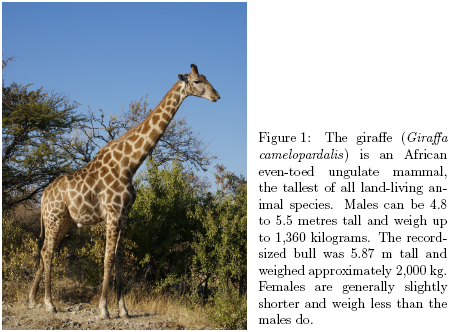
\includegraphics[width=0.48\textwidth]{./ingles/Latex_example_sidecap.jpg}
%  \end{center}
%\end{wrapfigure}

\begin{description}
\item[Nombre:] Balalaika
\item[Cristaleria:] Vaso largo (10oz / 300cc)
\item[M\'etodo de elaboraci\'on:] Batido
\item[Decoraci\'on:] Sin decoraci\'on.
\end{description}

\begin{table}[h]
\caption{Ingredientes y proporciones} 
\label{tab:fonts}
\begin{center}       
\begin{tabular}{|l|l|l|c|l|} %% this creates two columns
%% |l|l| to left justify each column entry
%% |c|c| to center each column entry
%% use of \rule[]{}{} below opens up each row
\hline
\rule[-1ex]{0pt}{3.5ex}  \textbf{Producto} & \textbf{Bebida} & \textbf{Marca} & \textbf{Volumen} & \textbf{Fraccion}  \\
\hline
\rule[-1ex]{0pt}{3.5ex}  Aguardiente & Vodka 			& Wyborowa 		& 2 oz / 60 cc 	&  	\\
\hline
\rule[-1ex]{0pt}{3.5ex}  Licor 		& Triple Sec 	& Cointreau 				& 1 1/2 oz / 45 cc 		&  	\\
\hline
\rule[-1ex]{0pt}{3.5ex}  Fruta 		& Limon & Jugo	& 1 1/2 oz / 45 cc		& 	\\
\hline

\end{tabular}
\end{center}
\end{table} 
\bigskip 

%%-----------------------------------------------------------
\subsubsection{Formato de elaboraci\'on} 
\label{sec:title}
\bigskip 
\begin{center}
\begin{enumerate}
\item Colocar en una coctelera una pala de hielo.
\item Servir los ingredientes en la misma.
\item Batir hasta que la coctelera est\'e helada.
\item Servir sin filtro en el vaso de trago largo.

\end{enumerate}
\end{center}
\bigskip 
\bigskip 
%%%%%%%%%%%%%%%%%%%%%%%%%%%%%%%%%%%%%%%%%%%%%%%%%%%%%%%%%%%%%

\subsubsection{Notas}
\bigskip 
\begin{center}
\raggedright{}Servir con sorbete.
\end{center} 

%\subsubsection{Informaci\'on extra}
\bigskip
%\begin{center}
\medskip 
%\raggedright{ \textbf{Or\'igenes de este trago}} \\ 
\medskip


%\end{center}
\newpage

\newpage
\bigskip \bigskip \bigskip
\subsection{Volga}
\bigskip 
\bigskip 
\subsubsection{Contenido}
\bigskip 
%\begin{wrapfigure}{r}{0.5\textwidth}
%  \begin{center}
%    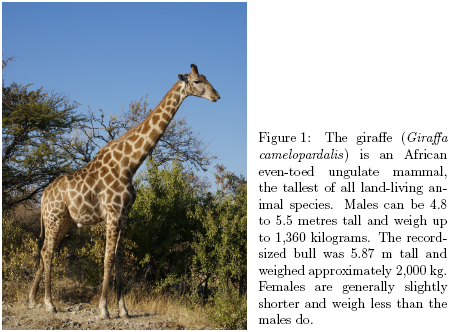
\includegraphics[width=0.48\textwidth]{./ingles/Latex_example_sidecap.jpg}
%  \end{center}
%\end{wrapfigure}

\begin{description}
\item[Nombre:] Volga
\item[Cristaleria:] Vaso Largo (10oz / 300cc)
\item[M\'etodo de elaboraci\'on:] Directo
\item[Decoraci\'on:] Sin decoraci\'on.
\end{description}

\begin{table}[h]
\caption{Ingredientes y proporciones} 
\label{tab:fonts}
\begin{center}       
\begin{tabular}{|l|l|l|c|l|} %% this creates two columns
%% |l|l| to left justify each column entry
%% |c|c| to center each column entry
%% use of \rule[]{}{} below opens up each row
\hline
\rule[-1ex]{0pt}{3.5ex}  \textbf{Producto} & \textbf{Bebida} & \textbf{Marca} & \textbf{Volumen} & \textbf{Fraccion}  \\
\hline
\rule[-1ex]{0pt}{3.5ex}  Aguardiente & Vodka 			& Wyborowa 		& 2 1/2 oz / 85 cc 	&  	\\
\hline
\rule[-1ex]{0pt}{3.5ex}  Licor 		& Menta	 	& Bols		& 1 oz / 30 cc 		&  	\\
\hline
\rule[-1ex]{0pt}{3.5ex}  Gaseosa	& Agua T\'onica 	& Schweppes 				& 5 oz / 150 cc		& 	\\
\hline

\end{tabular}
\end{center}
\end{table} 
\bigskip 

%%-----------------------------------------------------------
\subsubsection{Formato de elaboraci\'on} 
\label{sec:title}
\bigskip 
\begin{center}
\begin{enumerate}
\item Colocar el vodka y luego el licor en un vaso de trago largo.
\item Colocar las 5 oz de t\'onica, y rellenar con hielo picado.
\end{enumerate}
\end{center}
\bigskip 
\bigskip 
%%%%%%%%%%%%%%%%%%%%%%%%%%%%%%%%%%%%%%%%%%%%%%%%%%%%%%%%%%%%%

\subsubsection{Notas}
\bigskip 
\begin{center}
\raggedright{}Servir con sorbete.
\end{center} 
\newpage

\newpage
\bigskip \bigskip \bigskip
\subsection{Nueva Rusia}
\bigskip 
\bigskip 
 
\subsubsection{Contenido}
\bigskip 
\begin{description}
\item[Nombre:] Nueva Rusia
\item[Cristaleria:] Shot (3oz / 90cc)
\item[M\'etodo de elaboraci\'on:] Directo
\item[Decoraci\'on:] Sin decoración.
\end{description}

\begin{table}[h]
\caption{Ingredientes y proporciones}
\label{tab:fonts}
\begin{center}       
\begin{tabular}{|l|l|l|c|l|} %% this creates two columns
%% |l|l| to left justify each column entry
%% |c|c| to center each column entry
%% use of \rule[]{}{} below opens up each row
\hline
\rule[-1ex]{0pt}{3.5ex}  \textbf{Producto} & \textbf{Bebida} & \textbf{Marca} & \textbf{Volumen} & \textbf{Fraccion}  \\
\hline
\rule[-1ex]{0pt}{3.5ex}  Jarabe & Granadina		& Cusenier 	& 1 oz / 30 cc 	&  	\\
\hline
\rule[-1ex]{0pt}{3.5ex}  Licor		& Blue Curacao 	& Bols		& 1 oz / 30 cc 	& 	\\
\hline
\rule[-1ex]{0pt}{3.5ex}  Aguardiente		& Vodka 	& Wyborowa		& 1 oz / 30 cc 	& 	\\

\end{tabular}
\end{center}
\end{table} 
\bigskip 

%%-----------------------------------------------------------
\subsubsection{Formato de elaboraci\'on} 
\label{sec:title}
\bigskip 
\begin{center}
\begin{enumerate}
\item Servir en un vaso de shot los ingredientes.
\item Es muy importante respetar el orden de los mismos, ya que la idea del trago es formar la bandera rusa en el shot.
\item Servir primero la granadina, luego, lentamente el blue curacao, y finalmente el vodka.
\end{enumerate}
\end{center}
\bigskip \bigskip 
\bigskip 
%%%%%%%%%%%%%%%%%%%%%%%%%%%%%%%%%%%%%%%%%%%%%%%%%%%%%%%%%%%%%

\subsubsection{Notas}
\bigskip 
\begin{center}
\raggedright{}Servir sin sorbete.
\end{center} 
\bigskip \bigskip \bigskip 

\end{center}

\end{document} 